\usetikzlibrary{fit,arrows}
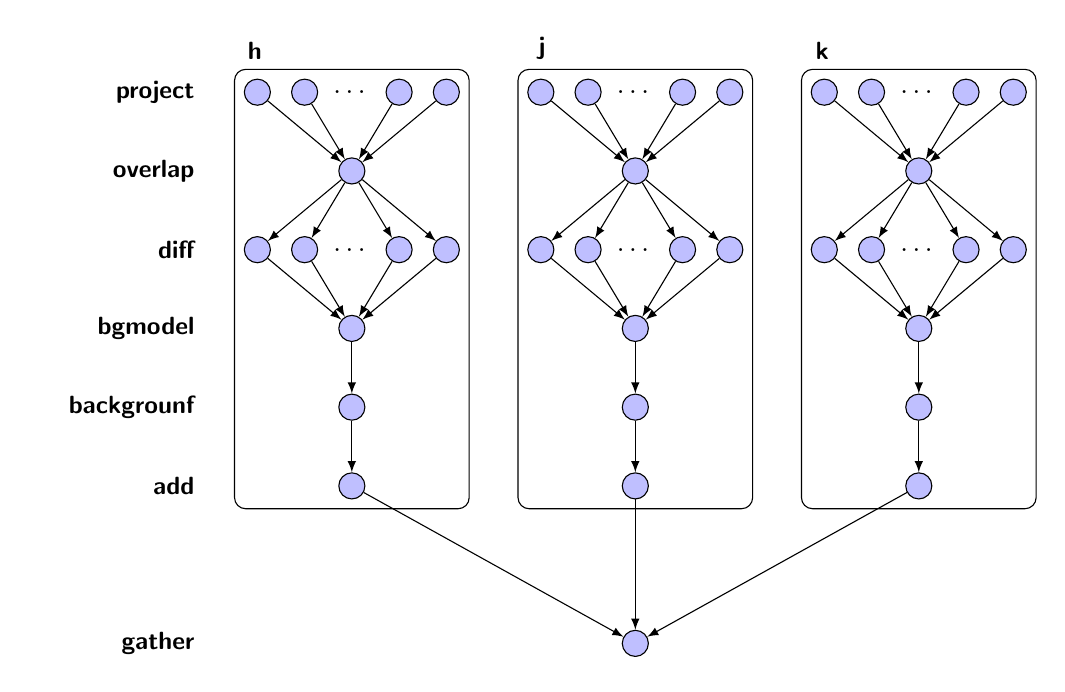
\begin{tikzpicture}[x=6mm,y=-10mm,
task/.style={%
 fill=blue!25,
draw,circle
},
level/.style={%
  font={\sffamily\bfseries\color{black} \fontsize{9pt}{12}\selectfont},
  align=right,
  text width=20mm
},
dot/.style={%
circle
}
]
%levels
\node[level] at (0,0)(Lproj){project};
\node[level] at (0,1)(Loverlap){overlap};
\node[level] at (0,2)(Ldiff){diff};
\node[level] at (0,3)(Lbgm){bgmodel};
\node[level] at (0,4)(Lbg){backgrounf};
\node[level] at (0,5)(Ladd){add};
\node[level] at(0,7)(Lgather){gather};
%%Gather node
\node[task,shift={(9,0)}]at(2,7)(gather){};
%%Loop HJK
\foreach \n [count=\i from 0] in {h,j,k}
{%
\begin{scope}[shift={(3+6*\i,0)}]
% 1 node per group
\node[task]at(2,1)(\i_overlap){};
\node[task]at(2,3)(\i_bgm){};
\node[task]at(2,4)(\i_bg){};
\node[task]at(2,5)(\i_add){};
%% 4 node per group
\foreach \y in {0,1,3,4}
{%
\node[task]at(\y,0)(\i_p_\y){};
\node[task]at(\y,2)(\i_d_\y){};
\draw[-{latex}](\i_p_\y)--(\i_overlap);
\draw[-{latex}](\i_overlap)--(\i_d_\y);
\draw[-{latex}](\i_d_\y)--(\i_bgm);
}
%%4 groups elipsis
\foreach \y in {0,2}
{%
\node[dot]at(2,\y){\ldots};
}
%%single deps
\draw[-{latex}](\i_bgm)--(\i_bg);
\draw[-{latex}](\i_bg)--(\i_add);
%%HJK boxes
\node[rounded corners,draw,fit=(\i_add)(\i_p_0)(\i_p_4),label={[font={\sffamily\bfseries\color{black}\fontsize{9pt}{12}\selectfont}]110:\n}]{};
\end{scope}
%% Gather deps
\draw[-{latex}](\i_add)--(gather);
}
\end{tikzpicture}